\begin{wrapfigure}[14]{r}{0.45\textwidth}
\centering
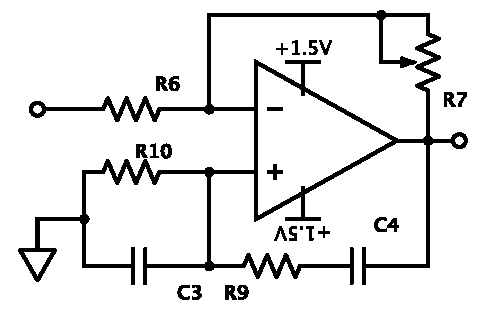
\includegraphics[width=.35\textwidth]{../E08/latex/osc.pdf}
\caption{Schema dell'oscillatore a ponte di Wien senza regolazione del guadagno.}
\label{cir8:without_lamp}
\end{wrapfigure}

\subsection{Oscillatore a ponte di Wien}

L'idea alla base dell'oscillatore a ponte di Wien è quella di sfruttare la selezione in frequenza di un filtro passa banda - il ponte di Wien - caratterizzato da avere il massimo guadagno per una determinata frequenza $f_0$.

Sappiamo inoltre che all'accensione dell'alimentazione del circuito si crea una forma d'onda che contiene virtualmente tutte le frequenze e pertanto anche $f_0$.

Ciò significa che, imponendo unitario il guadagno massimo del circuito, si otterrà un circuito che oscilla con ampiezza costante a $f_0$, con l'ampiezza data dall'ampiezza iniziale.

Lo schema in Figura \ref{cir8:without_lamp} presenta il circuito con amplificazione massima unitaria.
Come si può vedere esso è composto da un opamp con due rami di retroazione negativa e positiva.
Il ramo di feedback positivo è dato dal ponte di Wien mentre quello negativo è composto da un partitore resistivo.

Analizzando il circuito per $\omega_0=2\pi f_0=\frac{1}{RC}$ ($s=\frac{j}{RC}$) otteniamo dai due partitori:

\begin{equation}
  \begin{array}{lr}
	V^+_{f_0} = \frac{Z_{//}}{Z_1 + Z_{//}}V_{out} = \frac{1}{3}V_{out}\\
	V^-_{f_0} = \frac{R_1}{R_1+R_2}V_{out}
  \end{array} \bigg\}
\quad dove \quad %\intertext{dove}
\Bigg\{
  \begin{array}{lr}
	Z_1 := \frac{sRC+1}{sC}\\
	Z_{//} := \frac{R}{1+sRC}\\
	s = s_0 = \frac{2\pi}{RC}
  \end{array}
\end{equation}

Inserendo $V^+$ e $V^-$ nell'espressione del guadagno di un opamp si ottiene
\vspace{-2mm}
\begin{equation}
	V_{out,f_0} = A_{ol}\left( V^+_{f_0} - V^-_{f_0} \right) = A_{ol}\left(\frac{R_1}{R_1+R_2} - 1/3\right)V_{out,f_0}
\end{equation}
\vspace{-4mm}
da cui, per $A_{ol} \rightarrow \infty$, semplificando $V_{out,f_0}$

\begin{equation}
	R_2 = 2 R_1
\end{equation}

Utilizzando questi componenti otteniamo pertanto un sistema che oscilla alla frequenza $f_0$.
La problematica di tale circuito è però che non abbiamo il controllo dell'ampiezza con cui esso oscilla.

\subsubsection*{Controllo automatico del guadagno}

\begin{wrapfigure}[14]{l}{0.45\textwidth}
\centering
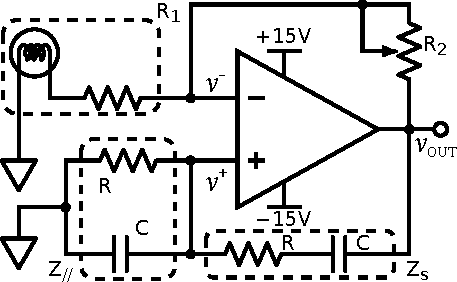
\includegraphics[width=.35\textwidth]{../E08/latex/osc_w_lamp.pdf}
\caption{Schema dell'oscillatore a ponte di Wien con regolazione del guadagno ottenuta mediante una lampadina a filamento.}
\label{cir8:with_lamp}
\end{wrapfigure}

La configurazione precedente è detta autoinnescante, cioè basta alimentare l'opamp affinché il circuito inizi ad oscillare.
Per avere un innesco certo è però necessario che il guadagno totale del circuito sia \textit{inizialmente} maggiore di \num{1}.

Per fare ciò si sostituisce la resistenza $R_1$ con una lampadina a filamento (il nuovo circuito è proposto in Figura \ref{cir8:with_lamp}).
Essa infatti possiede una coefficiente di temperature postivo che ne aumenta la resistenza con l'aumento temperatura, generato per effetto joule dalla corrente.

Inizialmente la resistenza sarà più fredda e pertanto il guadagno del circuito sarà maggiore di \num{1}, innescando l'oscillazione.
Con il passaggio di corrente nella lampadina, essa si scalderà e aumenterà la propria resistenza, diminuendo il guadagno portandolo a valori inferiori di \num{1}.
Ciò porterà il circuito a stabilizzarsi con un guadagno unitario e pertanto a generare un'oscillazione di frequenza $f_0$ di ampiezza costante.

\begin{figure}[htpc]
\centering
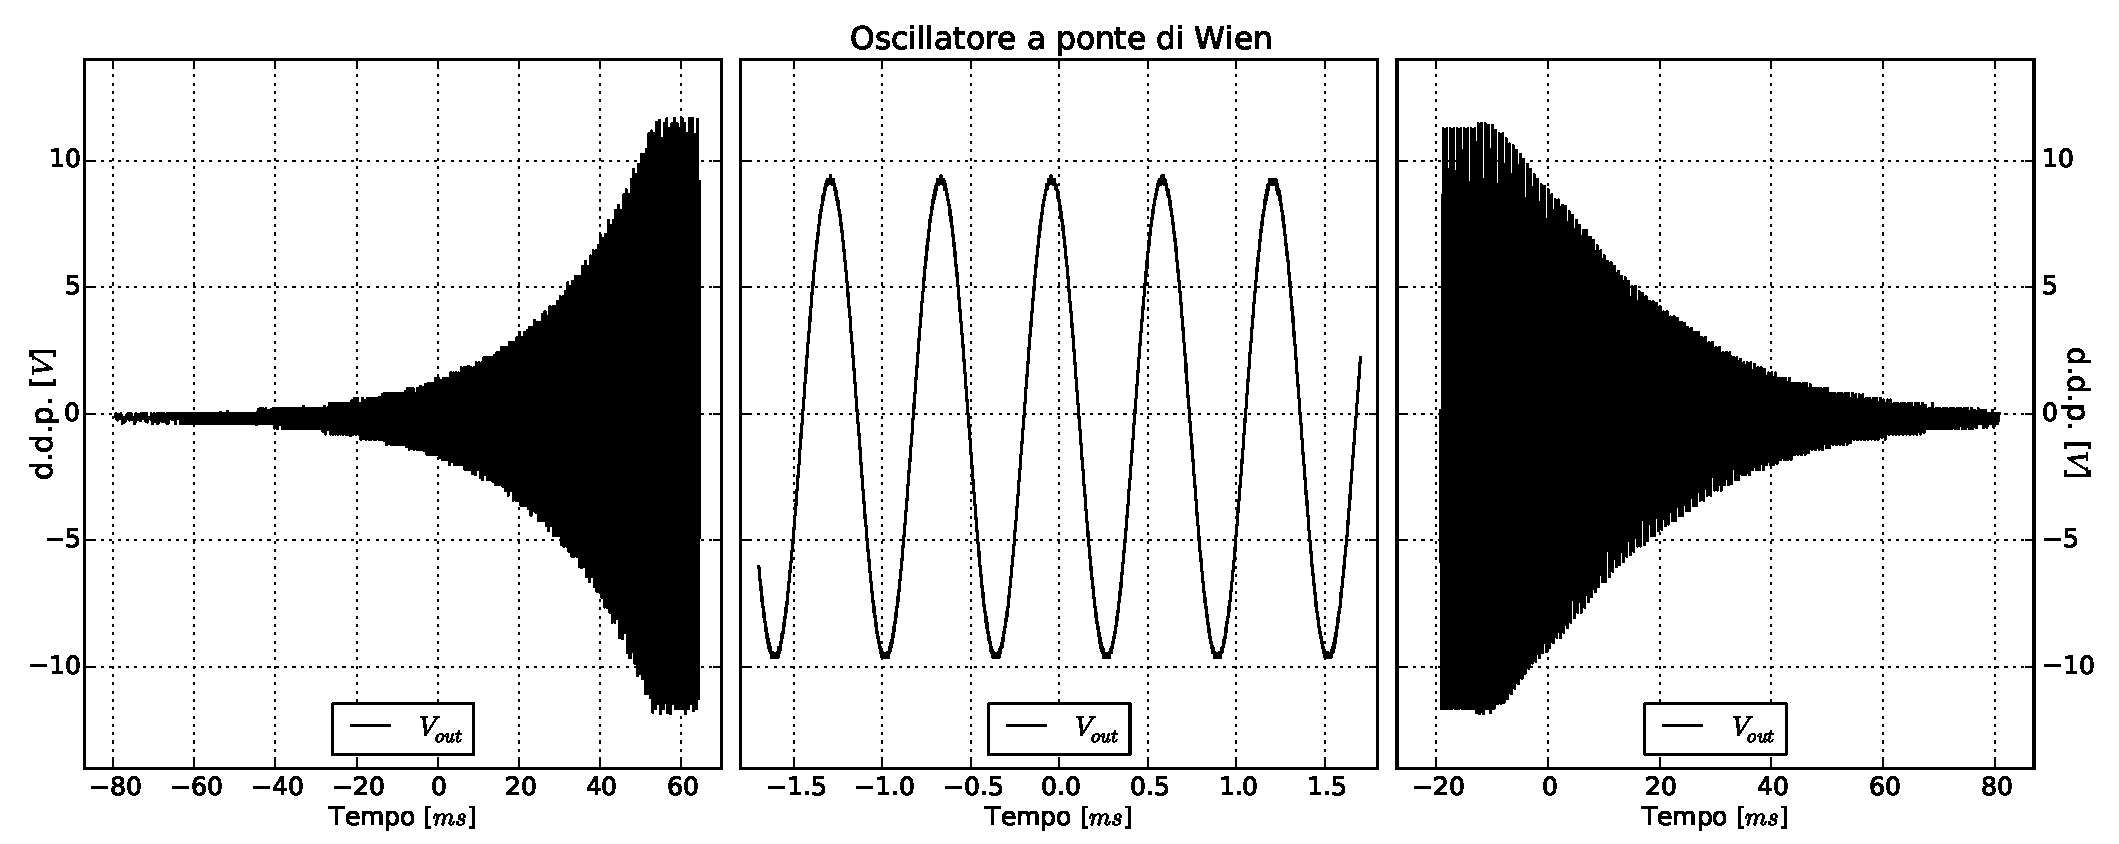
\includegraphics[width=.95\textwidth]{../E08/latex/wien.pdf}
\caption{Risposta del circuito oscillatore, nel grafico a sinistra in guadagno è maggiore di \num{1}, nel grafico centrale il guadagno è stabile, nel grafico a destra il guadagno è inferiore di \num{1}.}
\label{fig8:wien}
\end{figure}
